\documentclass[11pt]{article}
\usepackage{lscape}
\usepackage{amsmath,amssymb}
\usepackage{amsthm}
\usepackage{float}
\usepackage{booktabs}
\usepackage{graphicx}
\usepackage{comment}
\usepackage{bm}
\usepackage{gensymb}
\allowdisplaybreaks[4]
\usepackage{geometry}
\geometry{margin=1in}
\usepackage{setspace}
\usepackage{siunitx}
\usepackage{enumitem}
\usepackage{dsfont}

\usepackage{graphics}


\usepackage[utf8x]{inputenc}
\usepackage{bm}

\usepackage{hyperref}
\hypersetup{
    colorlinks=true,
    citecolor = blue,
    linkcolor=blue,
    filecolor=magenta,           
    urlcolor=cyan,
}


\theoremstyle{plain}
\newtheorem{thm}{Theorem}[section]
\newtheorem{claim}{Claim}
\newtheorem{lem}{Lemma}
\newtheorem{prop}{Proposition}
\newtheorem{pro}{Property}
\newtheorem{cor}{Corollary}
\newtheorem{ass}{Assumption}

\theoremstyle{definition}
\newtheorem{defn}{Definition}
\newtheorem{exmp}{Example}
\newtheorem{rmk}{Remark}

\usepackage{algpseudocode,algorithm}
\algnewcommand\algorithmicinput{\textbf{Input:}}
\algnewcommand\algorithmicoutput{\textbf{Output:}}
\algnewcommand\INPUT{\item[\algorithmicinput]}
\algnewcommand\OUTPUT{\item[\algorithmicoutput]}



\usepackage[labelfont=bf]{caption}

\setcounter{table}{1}
\usepackage{multirow}
\usepackage{tabularx}

\def\fixme#1#2{\textbf{[FIXME (#1): #2]}}

 

\newcommand*{\KeepStyleUnderBrace}[1]{%f
  \mathop{%
    \mathchoice
    {\underbrace{\displaystyle#1}}%
    {\underbrace{\textstyle#1}}%
    {\underbrace{\scriptstyle#1}}%
    {\underbrace{\scriptscriptstyle#1}}%
  }\limits
}
\usepackage{mathtools}
\mathtoolsset{showonlyrefs=true}


\usepackage{hyperref}
\hypersetup{colorlinks=true}
\usepackage[parfill]{parskip}
\usepackage{bm}
\onehalfspacing

\usepackage{multirow}

\newcommand{\newnorm}[1]{\left\lVert#1\right\rVert}
\usepackage{enumitem}
\newcommand{\Hnorm}[1]{\left\lVert#1\right\rVert_{\tH_\alpha}}
%%%%%%%%%%%%%%%%%%%%%%%%%%%%%%%%%%%%%%%%%%%%%%%%%%%%%%%%%%%%%%%%%%%%%
%%             Math Symbols
%%%%%%%%%%%%%%%%%%%%%%%%%%%%%%%%%%%%%%%%%%%%%%%%%%%%%%%%%%%%%%%%%%%%%

%%               Bold Math
\input macros.tex
\def\refer#1{\emph{\color{blue}#1}}
\begin{document}
\begin{center}
{\Large \bf NIPS data analysis} \\
Miaoyan Wang, Jan 14, 2021
\end{center}

The NIPS dataset~\cite{globerson2007euclidean} records the counts of words in 2,483 papers published from 1987 to 2003. We focus on the top 100 authors, 200 most frequent words, and normalize each word count by log transformation with pseudocount 1. The resulting dataset is an order-3 tensor $\tY\in\mathbb{R}^{100\times 200\times 17}$, where the entry $\tY(i,j,k)$ represents the log count of word $i$ by author $j$ in year $k$. 


We first investigate the prediction accuracy of tensor completion. Table~\ref{tab:NIPS} compares the performance of our method, low-rank CP decomposition, and naive imputation by sample average. The reported MAE is averaged over five runs of cross-validation, with 20\% entries for testing and 80\% for training. We find that our method substantially outperforms the classical low-rank method for every $r$ in the considered range. Further increment of rank appears to have little effect on the performance; doubling the rank to $r=20$ yields only 5\% relative deduction in MAD (see Appendix). In contrast, the low-rank CPT exhibits poor prediction even at a relatively high rank. The comparison highlights the advantage of our method in achieving accuracy while maintaining low complexity. In addition, the two tensor methods outperform the naive imputation, implying the necessity of incorporating tensor structure in the analysis. 

\begin{table}[H]
\centering
\begin{tabular}{c|ccccc}
Method & $r = 3$ & $r = 6$ & $r=9$ & $r=12$&$r=15$ \\
\hline
NonparaT (Ours) & {\bf 0.18}(0.002) & {\bf 0.16}(0.002) & {\bf 0.15}(0.001)& {\bf 0.14}(0.001)&{\bf 0.13}(0.001)\\
 \hline
Low-rank CPT &0.22(0.004) & 0.20(0.007) & 0.19(0.007)&0.17(0.007)&0.17(0.007)\\
  \hline
Naive imputation (Baseline)& \multicolumn{4}{c}{0.32(.001)}\\
\end{tabular}
\caption{Prediction accuracy measured in MAE in the NIPS data analysis. The reported MAEs are averaged over five runs of cross-validation, with standard errors in parentheses. For low-rank CPT, we use R function {\tt rTensor} with default hyperparameters, and for our method, we set $H=20$.}\label{tab:NIPS}
\end{table}

\vspace{-.5cm}
\begin{figure}[H]
\centering
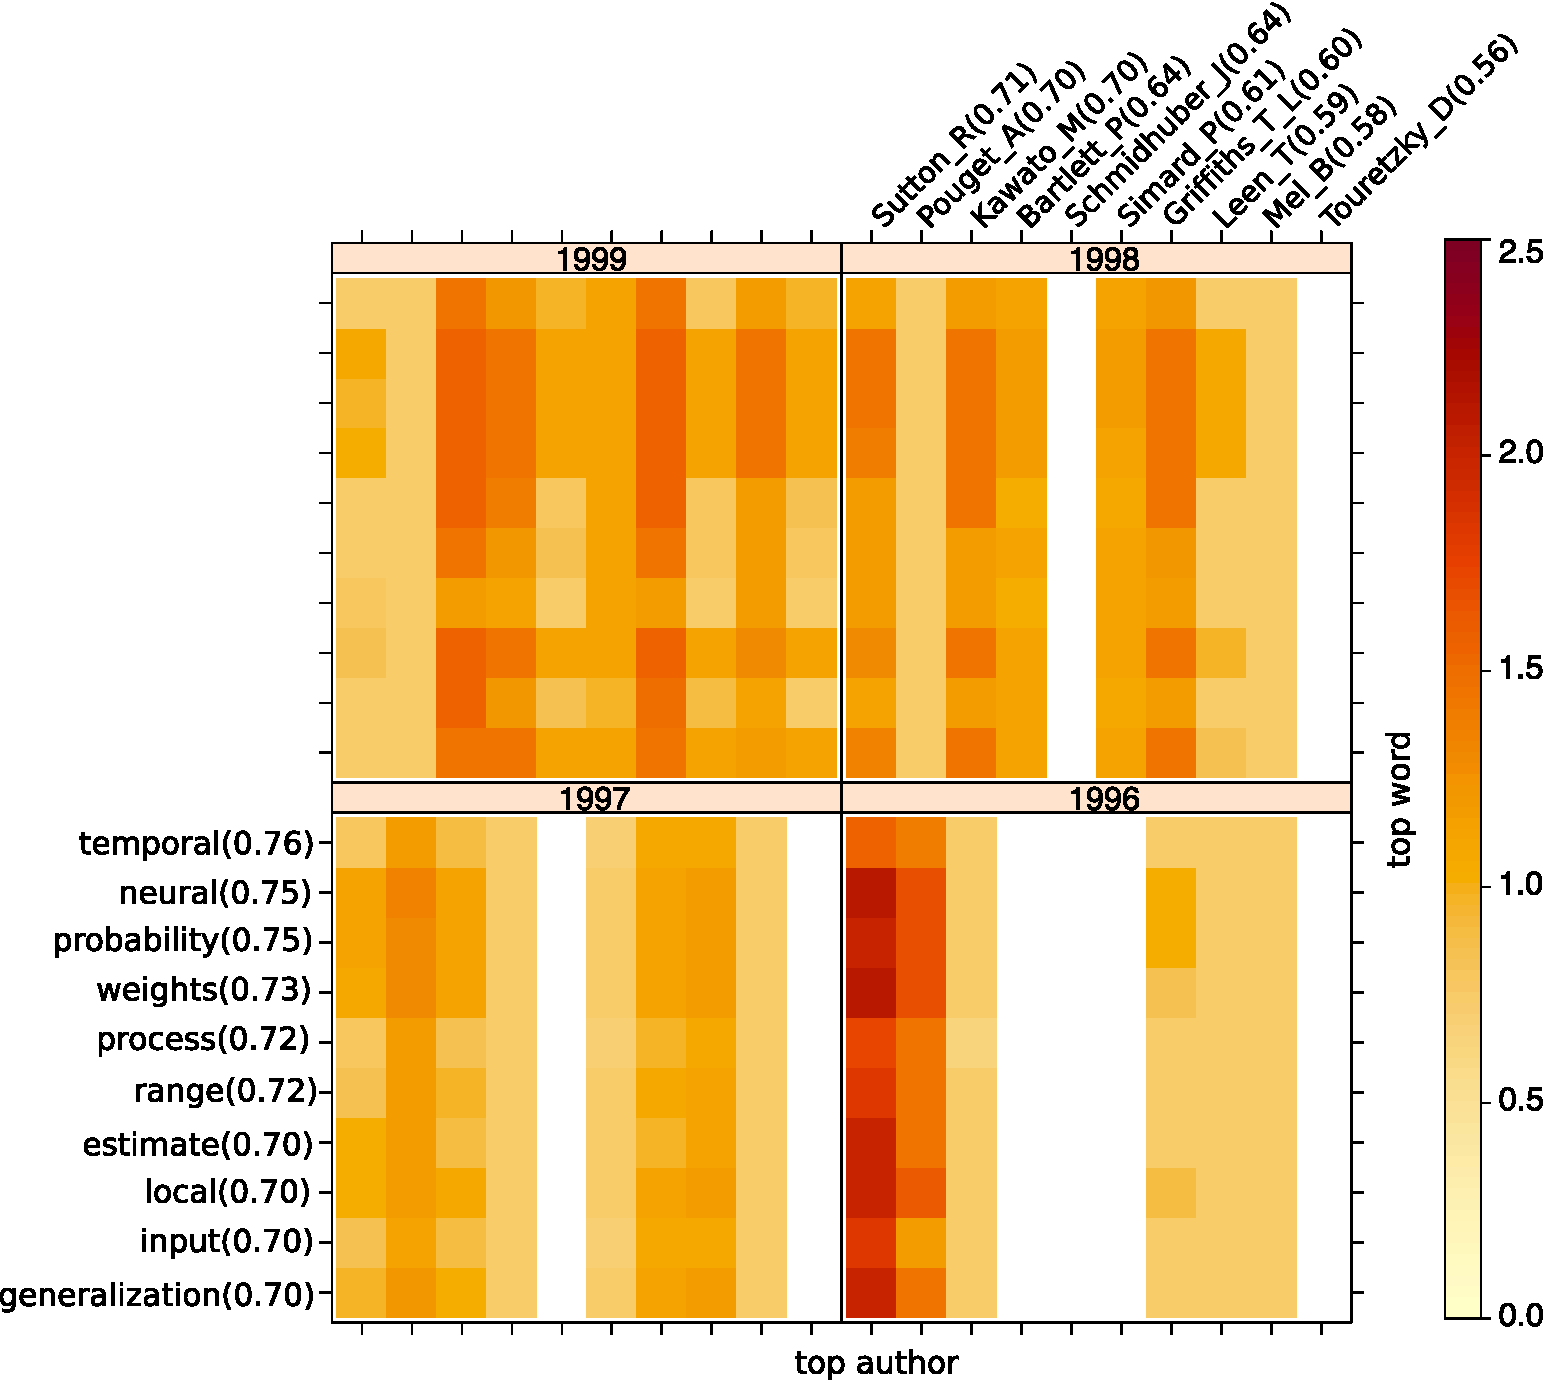
\includegraphics[width=.45\textwidth]{signal.pdf}
\caption{Estimated signal tensor with top authors and words in the years 1996-1999. Gray regions indicate no publication for the author in the specific year. Authors and words are ranked by marginal averages based on $\hat \Theta$, where the marginal average is denoted in the parentheses.}\label{fig:signal}
\end{figure}

Next, we examine the estimated signal tensor $\hat \Theta$ from our method with $r=10$ and the resolution parameter $H=20$. The result changes little with higher values of $r$ and $H$. We define $\hat \Theta(i,j,k)$ by our nonparametric estimate (6) if author $i$ publishes at least one paper in year $k$, and zero otherwise. Figure~\ref{fig:signal} illustrates the subtensor of $\hat \Theta$ consisting of top authors and words (after excluding generic words such as \emph{figure}, \emph{current}, etc). The detected patten is consistent with the active topics in the NIPS publication. For example, among the top words are \emph{temporal} (marginal mean = 0.76), \emph{neural} (0.75), and \emph{generalization} (0.70), whereas top authors are \emph{Richard Sutton} (0.71), \emph{Pouget\_A}(0.70), \emph{Kawato\_M} (0.70), and \emph{Bartlett Peter} (0.64). We also find strong heterogeneity among word occurrence across authors and years. For example, \emph{neural} and \emph{weights} are popular words for \emph{Tomas Griffiths} in 1998-1999, whereas \emph{temproal} occurs more often in Richard Sutton et al in 1996. The achieved denoising accuracy and pattern detection demonstrates the applicability of our method. {\color{red} (would be interesting to verify the specific papers in that year.) }




\bibliographystyle{plain}
\bibliography{tensor_wang.bib}
\end{document}
